\section{Baza de date cu filme}
În cadrul prezentei diserații a fost folosită ca bază de date pentru evaluarea experimentală baza oferită de grouplens \hyperlink{movielens}{[22]}. Aceștia pun la dispoziție mai multe seturi de date printre care:
\begin{enumerate}
	\item \textbf{MovieLens 20M Dataset}: conține 20 milioane de ratinguri oferite de 138 000 de utilizatori peste 27 000 de filme;
	\item \textbf{MovieLens 10M Dataset}: conține 10 milioane de ratinguri oferite de 72 000 de utilizatori peste 10 000 de filme;
	\item \textbf{MovieLens 1M Dataset}: conține 1 milion de ratinguri oferite de 6 000 de utilizatori peste 4 000 de filme.
\end{enumerate}

În evaluarea curentă a fost folosită cea mai recentă versiune de bază de date, actualizată la 9/2018, de dimensiune mică și anume \textit{ml-latest-small}. Această bază de date conține 100 000 de ratinguri și 3 600 de taguri aplicate peste 9 000 de filme de 600 de utilizatori. Această bază de date este un subset dintr-o bază de date cu 27 de milioane de ratinguri și 1 milion de taguri, aplicate peste 58 000 de filme de 280 000 de utilizatori.

Fiecare utilizator din \textit{ml-latest-small} a acordat ratinguri pentru cel puțin 20 de filme. Baza de date nu conține informații demografice, fiecare utilizator fiind reprezentat doar de un id.

Structura fișierelor din baza de date:
\begin{itemize}
	\item \textbf{ratings.csv}: fiecare linie din acest fișier reprezintă un rating dat de un utilizator unui film, fișierul având formatul $userId, movieId, rating, timestamp$, unde $timestamp$ reprezintă momentul de timp când a fost acordat ratingul. Fiecare rating este cuprins între 0 și 5, iar între ratinguri este un pas de 0.5;
	\item \textbf{movies.csv}: conține metadate despre filme precum titlul și genul. Formatul fișierului este următorul: $movieId, title, genres$. Titlul conține și anul de apariție a filmului sub forma \textit{Titlu (an)}. Genul poate fi unul sau mai multe dintre următoarele: \textit{Action, Adventure, Animation, Children's, Comedy, Crime, Documentary, Drama, Fantasy, Film-Noir, Horror, Musical, Mystery Romance, Sci-Fi, Thriller, War Western, (no genres listed)}.
	\item \textbf{links.csv}: conține referințele către site-urile movielens, imdb și themoviedb sub următorul format: $movieId,imdbId,tmdbId$, unde movieId este id-ul de pe site-ul movielens.
	\item \textbf{tags.csv}: fiecare linie conține un tag aplicat de un utilizator unui film, fișierul având următorul format $userId,movieId,tag,timestamp$. Fiecare tag este reprezentat de un cuvânt sau de o scurtă frază.
\end{itemize}

\section{Baza de date cu postere}
În ceea ce privește baza de date pentru postere, aceasta a fost construită în cadrul dezvoltării prezentei lucrări cu ajutorul a două elemente: fișierul de \textit{links} din setul de date \textit{ml-latest-small} și cu API-ul pus la dispoziție de către platforma \textbf{themoviedb.org} \hyperlink{themoviedb}{[24]}.

Procesul de construcție a acestui set de postere pentru filme poate fi rezumat pe pași după cum urmează:
\begin{enumerate}
	\item \textbf{Pasul 1}: extragerea id-urilor filmelor aferente platformei themoviedb.org;
	\item \textbf{Pasul 2}: pentru fiecare film se face un request către API pentru a lua lista de postere pentru filmul curent;
	\item \textbf{Pasul 3}: având adresele posterelor pentru filmul curent, se descarcă și se salvează posterele la dimensiunea originală într-un folder specific filmului.
\end{enumerate}
Din punct de vedere al implementării putem menționa funcțiile:
\begin{lstlisting}[language=Python, caption=\textit{Construcția setului de date cu postere}]
def get_tmdb_posters(tmdb_api_key, max_movie_posters=10):
    # pasul 1    
    tmdb_movies_id = get_tmdb_ids()
    # pasul 2 - 3
    download_images(tmdb_api_key, tmdb_movies_id, max_movie_posters)

# unde download_images are urmatoarea definitie:
def download_images(tmdb_api_key, tmdb_movies_id, max_movie_posters=10):
\end{lstlisting}
unde:
\begin{itemize}
	\item \textbf{tmdb\_api\_key} este api key-ul unic asociat unui cont pe platforma themoviedb.org care a solicitat acces la API-ul platformei;
	\item \textbf{max\_movie\_posters} definește care este numărul maxim de postere care va fi descărcat pentru un film. Numărul de postere descărcate poate fi mai mic în cazul în care nu sunt cel puțin max\_movie\_posters.
\end{itemize}

\begin{figure}[!tbp]
  \begin{subfigure}[b]{0.3\textwidth}
    
\includegraphics[width=9cm,height=5cm,keepaspectratio]{img_4_1}
  \end{subfigure}
  \hfill
  \begin{subfigure}[b]{0.3\textwidth}
    
\includegraphics[width=9cm,height=5cm,keepaspectratio]{img_4_2}
  \end{subfigure}
  \hfill
  \begin{subfigure}[b]{0.3\textwidth}
    
\includegraphics[width=9cm,height=5cm,keepaspectratio]{img_4_3}
  \end{subfigure}
  \hfill
  \begin{subfigure}[b]{0.3\textwidth}
    
\includegraphics[width=9cm,height=5cm,keepaspectratio]{img_4_4}
  \end{subfigure}
  \hfill
  \begin{subfigure}[b]{0.3\textwidth}
    
\includegraphics[width=9cm,height=5cm,keepaspectratio]{img_4_5}
  \end{subfigure}
  \hfill
  \begin{subfigure}[b]{0.3\textwidth}
    
\includegraphics[width=9cm,height=5cm,keepaspectratio]{img_4_6}
  \end{subfigure}
  \caption[Exemple de postere]{\textit{Exemplu de postere pentru filmul Paddington 2.}}
\end{figure}

\section{Rezultate clusterizare postere}

\subsection{Sanity check}
Pentru testarea validității clusterelor a fost creat un test de sanity check în care s-au luat opt filme și s-a încercat clasificarea lor în șapte clustere folosind caracteristicile extrase din rețelele preantrenate VGG16, VGG19, InceptionV3, ResNet50 și NASNet, clusterele sunt create cu kNN, iar evaluarea este făcută atât vizual cât și prin urmărirea evoluției metricii silhouette de la 2 la 7 clustere. Posterele de input pentru sanity check sunt prezentate în figura 4.2.
\begin{figure}[!h]
  \centering
  \begin{subfigure}[b]{0.48\textwidth}
    \includegraphics[width=\textwidth]{img_4_7}
  \end{subfigure}
  \hfill
  \begin{subfigure}[b]{0.48\textwidth}
    \includegraphics[width=\textwidth]{img_4_8}
  \end{subfigure}
    \hfill
  \begin{subfigure}[b]{0.48\textwidth}
    \includegraphics[width=\textwidth]{img_4_9}
  \end{subfigure}
  \hfill
  \begin{subfigure}[b]{0.48\textwidth}
    \includegraphics[width=\textwidth]{img_4_10}
  \end{subfigure}
  \hfill
  \begin{subfigure}[b]{0.48\textwidth}
    
\includegraphics[width=\textwidth]{img_4_11}
  \end{subfigure}
  \hfill
  \begin{subfigure}[b]{0.48\textwidth}
    
\includegraphics[width=\textwidth]{img_4_12}
  \end{subfigure}
    \hfill
  \begin{subfigure}[b]{0.48\textwidth}
    
\includegraphics[width=\textwidth]{img_4_13}
  \end{subfigure}
    \hfill
  \begin{subfigure}[b]{0.48\textwidth}
    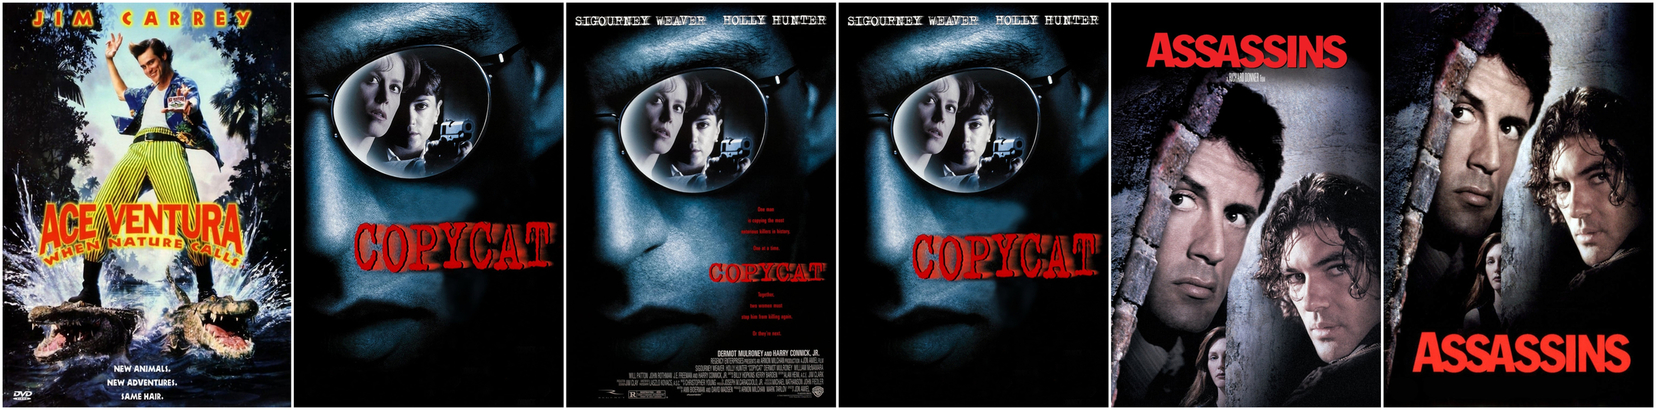
\includegraphics[width=\textwidth]{img_4_14}
  \end{subfigure}
      \hfill
  \begin{subfigure}[b]{0.3\textwidth}
    
\includegraphics[width=\textwidth]{img_4_15}
  \end{subfigure}
  \caption[Postere input sanity check]{\textit{Posterele de input pentru sanity check.}}
\end{figure}

Din punct de vedere al metricii de evaluare silhouette rezultatele se prezintă după cum urmează în figura 4.3, unde un scor silhouette mai mare reprezintă un rezultat mai bun.
\begin{figure}[!h]
	\centering
	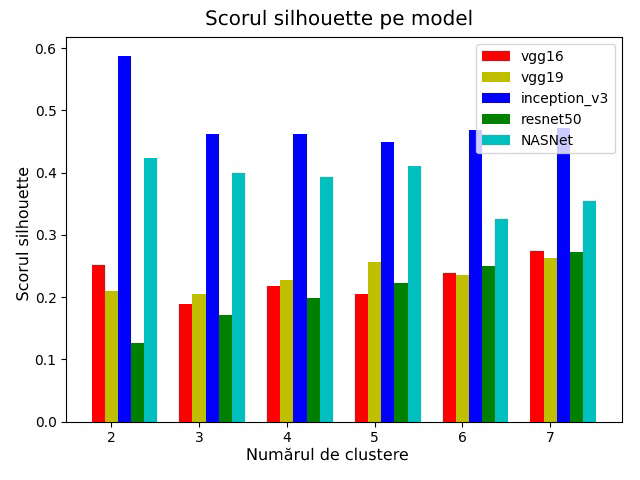
\includegraphics[max width=12cm,max height=12cm,keepaspectratio]{img_4_16}
	\caption[Silhouette score pentru clusterele din sanity check]{\textit{Silhouette score pentru clusterele din sanity check.}}
\end{figure} 
După cum se oberservă reţelele InceptionV3 şi NASNet au constant rezultate mai bune decât celelalte, cu un avantaj al reţelei InceptionV3. Această observaţie
fiind valabile pentru toate clusterele de la 2 la 7. Toate celelalte reţele sunt destul de
apropiate în rezultate în special începând cu clusterul 3 şi mai puţin la clusterul 2. Toate
celelalte reţele, cu excepţia ResNet50 au fluctuaţii. ResNet50 este singura care păstrează
în mod continuu trendul ascendent de la clusterul 2 până la clusterul 7.

Din punct de vedere vizual, rezultatatele clusterelor sunt prezentate în figurile 4.4 - 4.8.
\begin{figure}[!h]
  \centering
  \begin{subfigure}[t]{0.45\textwidth}
    \caption{cluster 1}
    
\includegraphics[width=\textwidth]{img_vgg16_c1}
  \end{subfigure}
  \hfill
  \begin{subfigure}[t]{0.45\textwidth}
    \caption{cluster 2}
    
\includegraphics[width=\textwidth]{img_vgg16_c2}
  \end{subfigure}
   \hfill
  \begin{subfigure}[t]{0.45\textwidth}
    \caption{cluster 3}
    
\includegraphics[width=\textwidth]{img_vgg16_c3}
  \end{subfigure}
  \hfill
  \begin{subfigure}[t]{0.45\textwidth}
    \caption{cluster 4}
    
\includegraphics[width=\textwidth]{img_vgg16_c4}
  \end{subfigure}
  \hfill
  \begin{subfigure}[t]{0.45\textwidth}
    \caption{cluster 5}
    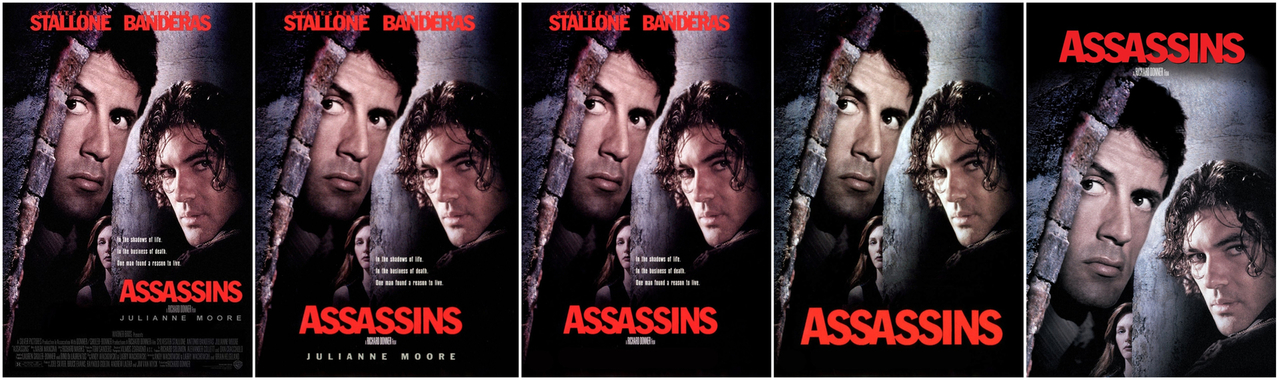
\includegraphics[width=\textwidth]{img_vgg16_c5}
  \end{subfigure}
  \hfill
  \begin{subfigure}[t]{0.45\textwidth}
    \caption{cluster 6}
    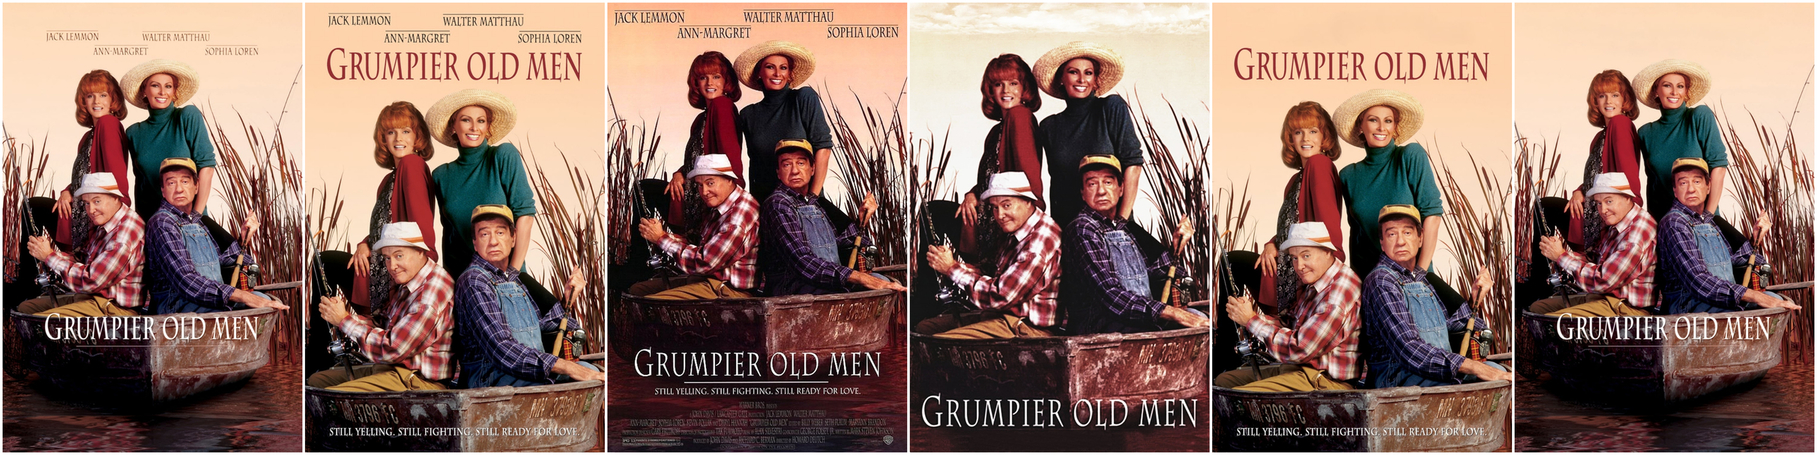
\includegraphics[width=\textwidth]{img_vgg16_c6}
  \end{subfigure}
    \hfill
  \begin{subfigure}[t]{0.45\textwidth}
    \caption{cluster 7}
    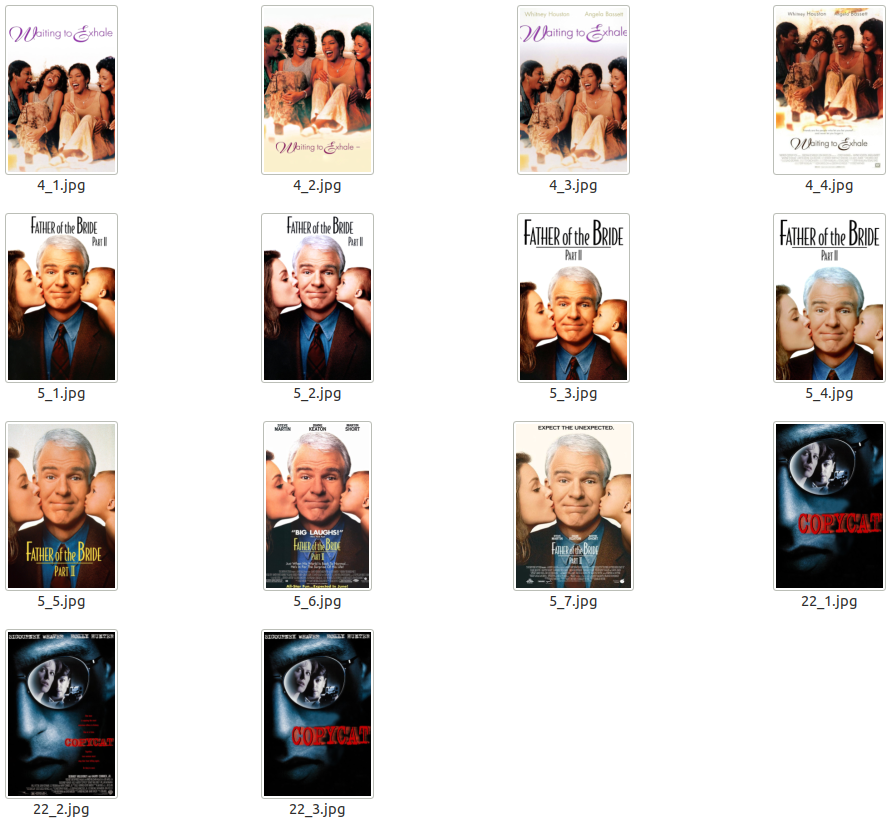
\includegraphics[width=\textwidth]{img_vgg16_c7}
  \end{subfigure}
  \caption[Rezultate sanity check pentru rețeaua VGG16]{\textit{Rezultate sanity check pentru rețeaua VGG16}}
\end{figure}

\begin{figure}[!h]
  \centering
  \begin{subfigure}[t]{0.45\textwidth}
	\caption{cluster 1}    
    
\includegraphics[width=\textwidth]{img_vgg19_c1}
  \end{subfigure}
  \hfill
  \begin{subfigure}[t]{0.45\textwidth}
    \caption{cluster 2}
    
\includegraphics[width=\textwidth]{img_vgg19_c2}
  \end{subfigure}
   \hfill
  \begin{subfigure}[t]{0.45\textwidth}
    \caption{cluster 3}
    
\includegraphics[width=\textwidth]{img_vgg19_c3}
  \end{subfigure}
  \hfill
  \begin{subfigure}[t]{0.45\textwidth}
    \caption{cluster 4}
    
\includegraphics[width=\textwidth]{img_vgg19_c4}
  \end{subfigure}
  \hfill
  \begin{subfigure}[t]{0.45\textwidth}
    \caption{cluster 5}
    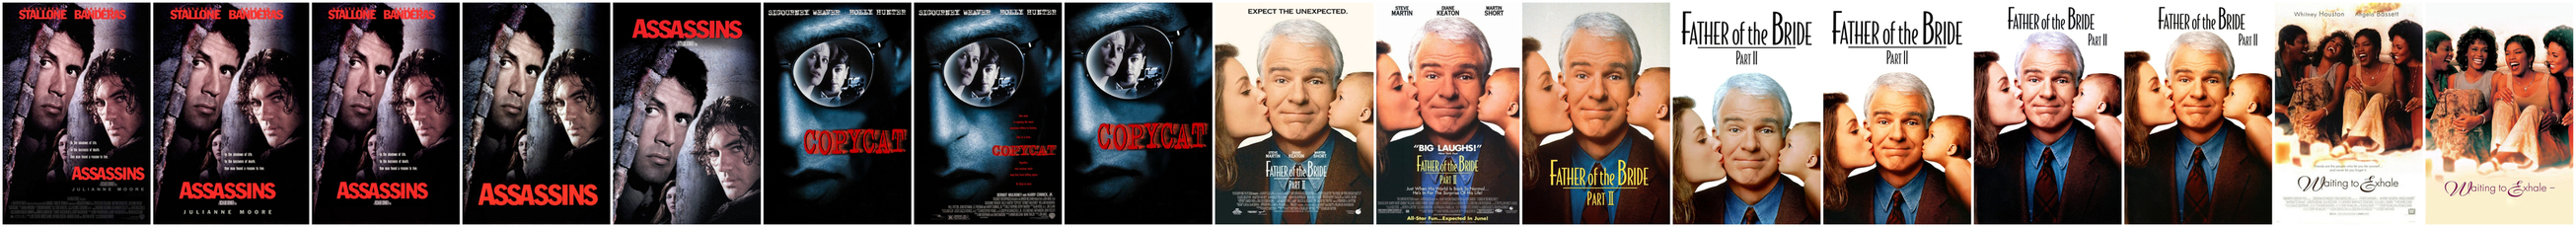
\includegraphics[width=\textwidth]{img_vgg19_c5}
  \end{subfigure}
  \hfill
  \begin{subfigure}[t]{0.45\textwidth}
    \caption{cluster 6}
    
\includegraphics[width=\textwidth]{img_vgg19_c6}
  \end{subfigure}
    \hfill
  \begin{subfigure}[t]{0.45\textwidth}
    \caption{cluster 7}
    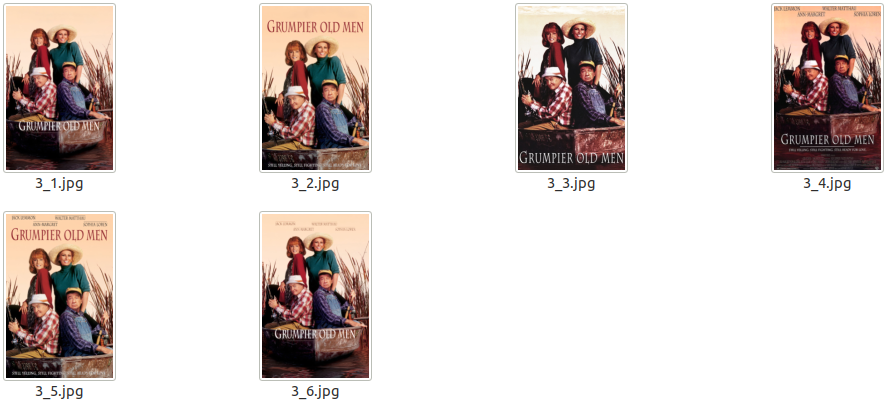
\includegraphics[width=\textwidth]{img_vgg19_c7}
  \end{subfigure}
  \caption[Rezultate sanity check pentru rețeaua VGG19]{\textit{Rezultate sanity check pentru rețeaua VGG19}}
\end{figure}

\begin{figure}[!h]
  \centering
  \begin{subfigure}[t]{0.45\textwidth}
    \caption{cluster 1}
    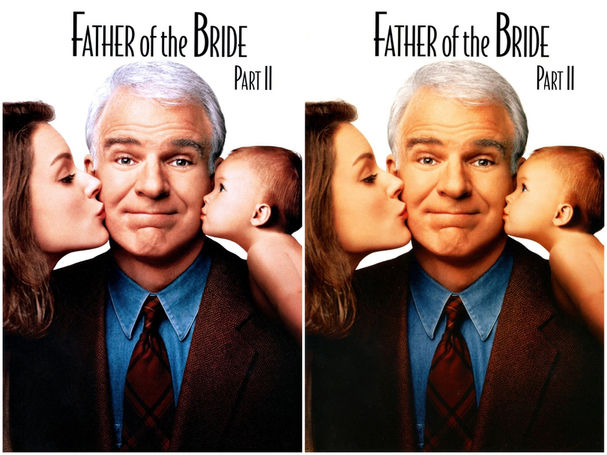
\includegraphics[width=\textwidth]{img_inceptionv3_c1}
  \end{subfigure}
  \hfill
  \begin{subfigure}[t]{0.45\textwidth}
    \caption{cluster 2}
    
\includegraphics[width=\textwidth]{img_inceptionv3_c2}
  \end{subfigure}
   \hfill
  \begin{subfigure}[t]{0.45\textwidth}
    \caption{cluster 3 - prima parte}
    
\includegraphics[width=\textwidth]{img_inceptionv3_c3_1}
  \end{subfigure}
  \hfill
  \begin{subfigure}[t]{0.45\textwidth}
    \caption{cluster 3 - a doua parte}
    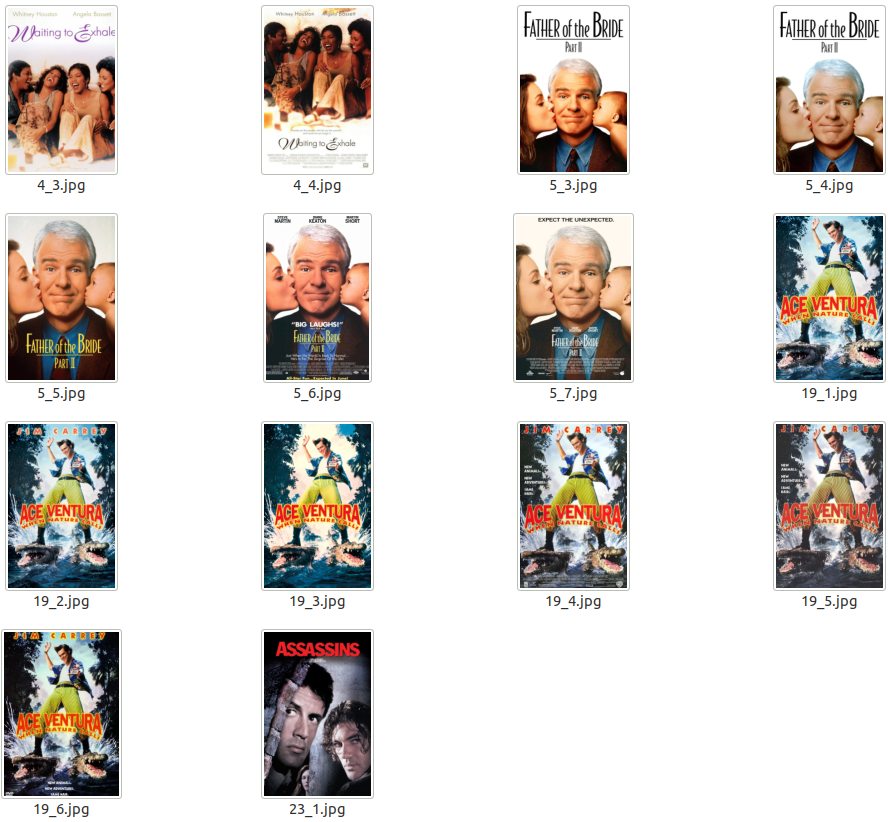
\includegraphics[width=\textwidth]{img_inceptionv3_c3_2}
  \end{subfigure}
  \hfill
  \begin{subfigure}[t]{0.45\textwidth}
    \caption{cluster 4}
    
\includegraphics[width=\textwidth]{img_inceptionv3_c4}
  \end{subfigure}
  \hfill
  \begin{subfigure}[t]{0.45\textwidth}
    \caption{cluster 5}
    
\includegraphics[width=\textwidth]{img_inceptionv3_c5}
  \end{subfigure}
  \hfill
  \begin{subfigure}[t]{0.45\textwidth}
    \caption{cluster 6}
    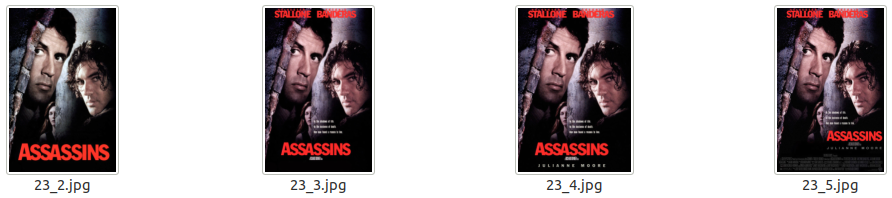
\includegraphics[width=\textwidth]{img_inceptionv3_c6}
  \end{subfigure}
    \hfill
  \begin{subfigure}[t]{0.45\textwidth}
    \caption{cluster 7}
    
\includegraphics[width=\textwidth]{img_inceptionv3_c7}
  \end{subfigure}
  \caption[Rezultate sanity check pentru rețeaua InceptionV3]{\textit{Rezultate sanity check pentru rețeaua InceptionV3}}
\end{figure}

\begin{figure}[!h]
  \centering
  \begin{subfigure}[t]{0.45\textwidth}
    \caption{cluster 1}
    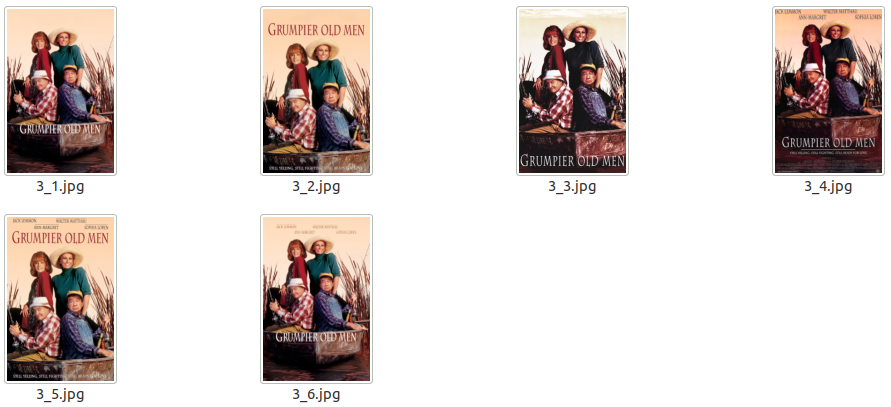
\includegraphics[width=\textwidth]{img_resnet50_c1}
  \end{subfigure}
  \hfill
  \begin{subfigure}[t]{0.45\textwidth}
    \caption{cluster 2}
    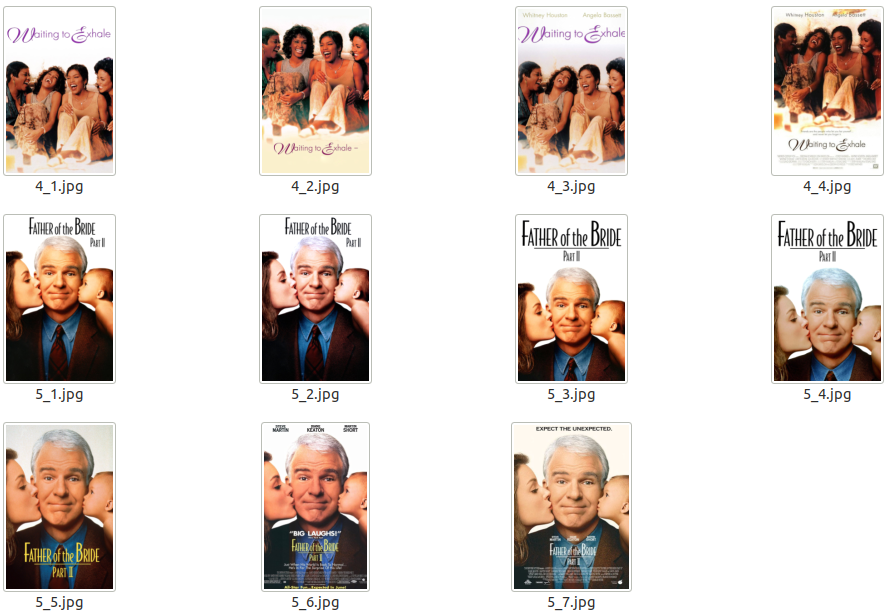
\includegraphics[width=\textwidth]{img_resnet50_c2}
  \end{subfigure}
   \hfill
  \begin{subfigure}[t]{0.45\textwidth}
    \caption{cluster 3}
    
\includegraphics[width=\textwidth]{img_resnet50_c3}
  \end{subfigure}
  \hfill
  \begin{subfigure}[t]{0.45\textwidth}
    \caption{cluster 4}
    
\includegraphics[width=\textwidth]{img_resnet50_c4}
  \end{subfigure}
  \hfill
  \begin{subfigure}[t]{0.45\textwidth}
    \caption{cluster 5}
    
\includegraphics[width=\textwidth]{img_resnet50_c5}
  \end{subfigure}
  \hfill
  \begin{subfigure}[t]{0.45\textwidth}
    \caption{cluster 6}
    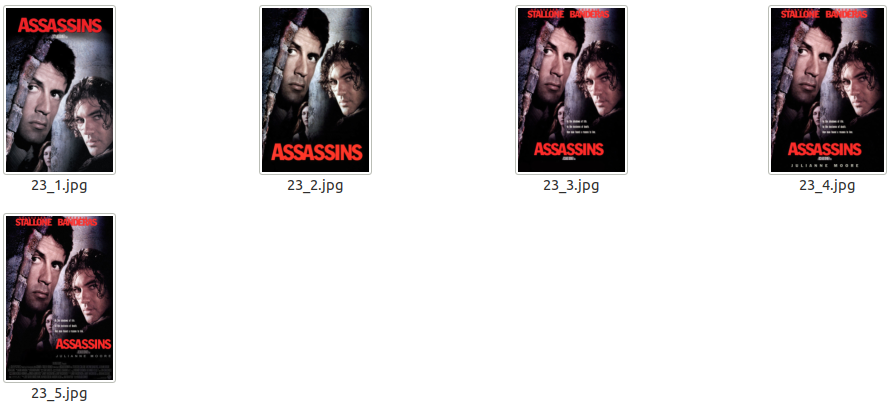
\includegraphics[width=\textwidth]{img_resnet50_c6}
  \end{subfigure}
    \hfill
  \begin{subfigure}[t]{0.45\textwidth}
    \caption{cluster 7}
    
\includegraphics[width=\textwidth]{img_resnet50_c7}
  \end{subfigure}
  \caption[Rezultate sanity check pentru rețeaua ResNet50]{\textit{Rezultate sanity check pentru rețeaua ResNet50}}
\end{figure}

\begin{figure}[!h]
  \centering
  \begin{subfigure}[t]{0.45\textwidth}
    \caption{cluster 1}
    
\includegraphics[width=\textwidth]{img_nasnet_c1}
  \end{subfigure}
  \hfill
  \begin{subfigure}[t]{0.45\textwidth}
    \caption{cluster 2}
    
\includegraphics[width=\textwidth]{img_nasnet_c2}
  \end{subfigure}
   \hfill
  \begin{subfigure}[t]{0.45\textwidth}
    \caption{cluster 3}
    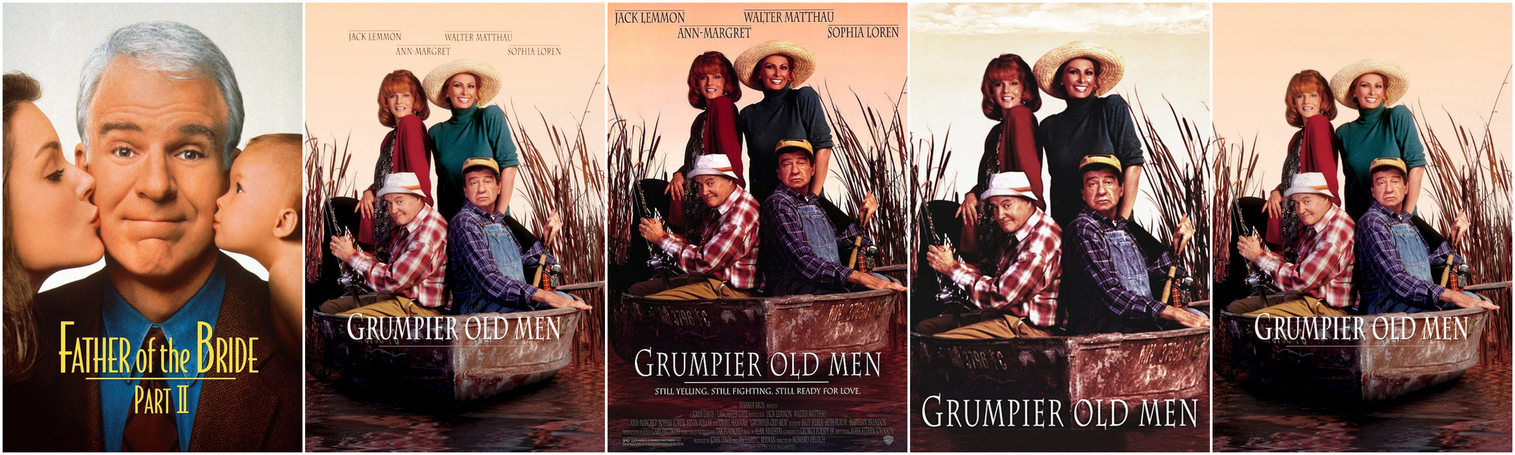
\includegraphics[width=\textwidth]{img_nasnet_c3}
  \end{subfigure}
  \hfill
  \begin{subfigure}[t]{0.45\textwidth}
    \caption{cluster 4}
    
\includegraphics[width=\textwidth]{img_nasnet_c4}
  \end{subfigure}
  \hfill
  \begin{subfigure}[t]{0.45\textwidth}
    \caption{cluster 5}
    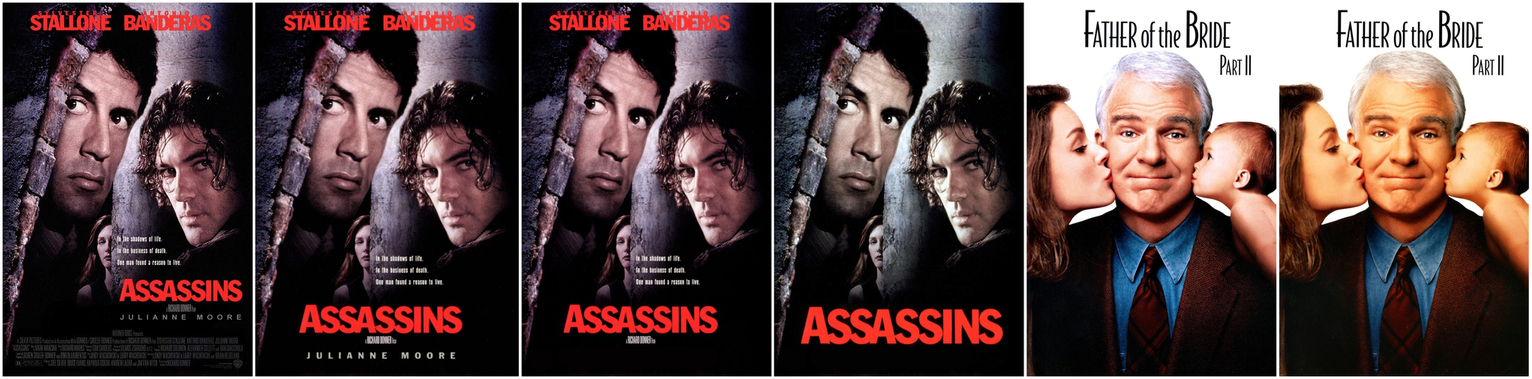
\includegraphics[width=\textwidth]{img_nasnet_c5}
  \end{subfigure}
  \hfill
  \begin{subfigure}[t]{0.45\textwidth}
    \caption{cluster 6}
    \includegraphics[width=\textwidth]{img_nasnet_c6}
  \end{subfigure}
    \hfill
  \begin{subfigure}[t]{0.45\textwidth}
    \caption{cluster 7}
    \includegraphics[width=\textwidth]{img_nasnet_c7}
  \end{subfigure}
  \caption[Rezultate sanity check pentru rețeaua NASNet]{\textit{Rezultate sanity check pentru rețeaua NASNet}}
\end{figure}

După cum se observă, din punct de vedere vizual doar rețeaua ResNet50 reușește să treacă acest sanity check clasificând sașe filme în șase clustere diferite, iar două filme în același cluster. Din punct de vedere vizual posterele celor două filme clasificate în același cluster sunt destul de similare având în prim plan mai multe persoane, predominant începând cu partea de jos a posterelor, iar in partea de sus fiind conținut alb, în general, cu text.

Observăm că deși InceptionV3 și NASNet aveau scoruri mai mari pe coeficientul silhouette, rețeaua ResNet50 are rezultate vizuale mai bune pe sanity check. De remarcat corelația dintre faptul că rețeaua ResNet50 este singura a cărui coeficient silhouette creștea de la un cluster la altul, ceea ce înseamnă că acele clustere deveneau din ce în ce mai bune pe măsură ce ne apropiam de numărul de clustere din realitate.

\FloatBarrier
\subsection{Rezultate generale}
Pentru evaluarea clusterelor (vezi figura 4.9) pe toate posterele filmelor, aproximativ 9 000, au fost eliminate din evaluare rețelele VGG16 și NASNet în baza rezultatelor prezentate în tabelul 3.1, în cazul rețelei VGG16 și a costului de memorie și timpului de execuție din timpul experimentelor, în cazul rețelei NASNet.
\begin{figure}[!h]
	\centering
	\includegraphics[max width=12cm,max height=12cm,keepaspectratio]{img_4_17}
	\caption[Scorul silhouette pe setul de date de postere]{\textit{Scorul silhouette pe setul de date de postere.}}
\end{figure} 
Se observă că rețeaua InceptionV3 are scorurile pentru toate clusterele de la 2 la 20 pozitive. Rețelele ResNet50 și VGG19 sunt negative, însă apropiate de 0 cu un avantaj de scoruri mai bune pentru rețeaua ResNet50.

În figurile 4.10 - 4.12 sunt prezentate rezultatele vizuale din trei clustere create cu rețeaua preantrenată ResNet50.
\begin{figure}[!h]
	\centering
	\includegraphics[max width=16cm,max height=12cm,keepaspectratio]{img_4_26}
	\caption[Cluster cu postere predominant negre]{Cluster cu postere predominant negre.}
\end{figure} 
\begin{figure}[!h]
	\centering
	\includegraphics[max width=16cm,max height=12cm,keepaspectratio]{img_4_27}
	\caption[Cluster cu postere predominant din filme de animație]{Cluster cu postere predominant din filme de animație.}
\end{figure} 
\begin{figure}[!h]
	\centering
	\includegraphics[max width=16cm,max height=12cm,keepaspectratio]{img_4_28}
	\caption[Cluster cu postere combinate]{\textit{Cluster cu postere combinate.}}
\end{figure} 

\section{Rezultate sistem de recomandare}
În continuare vom studia rezultatele obținute de metricile de evaluare \textbf{precizie@k} și \textbf{acuratețe} pe timp de antrenare în epoci, pe metadate folosite în antrenarea modelului și pe tipuri de rețele preantrenate cu care au fost generate clusterele posterelor. Toate mențiunile către parametrii optimi pentru o anumite configurație se referă la parametrii prezentați în tabelele 3.1 și 3.2.

Înainte de a prezenta rezultatele metricilor trebuie menționate două aspecte importante legate de configurația setului de date utilizat:
\begin{enumerate}
	\item ratingul minim pentru interacțiuni a fost setat la 3.5, ceea ce înseamnă că s-au folosit ca interacțiuni pozitive doar acele interacțiuni care au cel puțin acest rating;
	\item rezultatul maxim al metricii de precizie@k este direct influențat de numărul de interacțiuni dintre utilizatori și filme. Spre exemplu, dacă un utilizator are un număr total de 5 interacțiuni, iar metrica noastră de precizie are k-ul setat la 10, atunci rezultatul maxim pentru precizie@5 va fi 0.5, $50\%$, deoarece nu există mai multe de 5 interacțiuni pozitive pentru acel utilizator.
\end{enumerate}

În cazul împărțirii utilizate numărul de interacțiuni se prezintă după cum urmează:
\begin{itemize}
	\item pentru tot setul de date, numărul de interacțiuni pe utilizator: minim: 1; mediu: 101; maxim: 1459; utilizatori cu mai puțin de k=10 interacțiuni: 20 din 609 
	\item pentru setul de date de train, numărul de interacțiuni pe utilizator: minim: 1; mediu: 81; maxim: 1165; utilizatori cu mai puțin de k=10 interacțiuni: 38 din 609
	\item pentru setul de date de test, numărul de interacțiuni pe utilizator: minim: 1; mediu: 20; maxim: 294; utilizatori cu mai puțin de k=10 interacțiuni: 296 din 598
\end{itemize}

Rezultatele metricii de acuratețe sunt prezentate în figura 4.13 (a). Aceste rezultate sun obținute utilizând parametrii optimi din tabelul 3.1. Reamintim că toate clusterele folosite pentru obținerea parametrilor optimi din acest tabel au fost create folosind rețeaua VGG19.
\begin{figure}[!h]
  \begin{subfigure}[b]{0.5\textwidth}
    \includegraphics[width=\textwidth]{img_4_18}
    \caption{}
    \label{fig:f1}
  \end{subfigure}
  \hfill
  \begin{subfigure}[b]{0.5\textwidth}
    \includegraphics[width=\textwidth]{img_4_19}
    \caption{}
    \label{fig:f2}
  \end{subfigure}
  \caption[Comparație acuratețea modelului cu parametrii optimi pe tipuri de metadate]{\textit{Comparație acuratețea modelului cu parametrii optimi pe tipuri de metadate (a) și cu parametrii optimi pe tipuri de metadate cu număr setat de epoci (b).}}
\end{figure}
Principalele concluzii pe care le putem trage pe baza acestor grafice sunt următoarele:
\begin{itemize}
	\item modelul fără metadate are un start mai bun decât decât modelul cu genuri sau modelul cu genuri și cu clustere, însă acesta nu urcă prea mult pe durata perioadei de antrenare, astfel ajungând să aibă cel mai slab rezultat dintre toate cele patru variante de model testate;
	\item modelul cu metadatele de genuri are un start mai slab, fiind mai bun doar față de modelul în care se folosesc atât genurile cât și clusterele, însă, până la final, acest model obține un rezultat bun și apropiat de rezultatul modelului cu genuri și clustere. O altă mențiune importantă ar fi că acest model are o durată de antrenare mai mare față de toate celelalte modele;
	\item modelul cu metadatele de clustere are start mai bun și în același timp o perioadă de antrenare mai scurtă pentru a obține cel mai optim rezultat dintre toate modelele testate. Acuratețea obținută de acest model este peste acuratețea obținută de modelul fără metadate dar sub cea obținută de modelul cu genuri însă destul de apropiată de aceasta;
	\item cel mai bun rezultat din cadrul acestui experiment este obținut de modelul în care se folosesc atât metadatele de genuri cât și cele de clustere. Modelul are un start mai slab însă un rezultat final bun. Observăm că modul în care este obținut rezultatul este o combinație a avantajelor modelelor cu metadate de genuri și clustere. Pe de-o parte, acuratețea crește semnificativ față de modelul fără metadate și este apropiată de acuratețea modelului cu genuri. Pe de altă parte timpul necesar obținerii acelui rezultat optim este mai scăzut decât la modelul cu genuri, timp influențat de metadatele de clustere.
\end{itemize}

Concluzia principală a acestui experiment este că un model ce conține genuri și clustere are o performanță de până la $1\%$ în plus față de modelul fără metadate și mai mare față de oricare alt model, iar timpul necesar pentru obținerea acestei performanțe este mai mic în comparație cu cel mai apropiat model din punct de vedere al metricii evaluate.

Pentru a avea o imagine mai completă de cum se pot comporta aceste modele în timp am eliminat parametrul optimi găsit pe numărul de epoci și l-am setat pentru fiecare model la un număr de 300 de epoci. Iar după cum se observă în figura 4.13 (b) toate modele după punctul optim în care ating performanța maximă încep să scadă. Modelele fără metadate, cu metadatele de genuri și clustere au o scădere destul de lină în timp, pe când scăderea este mai accelărată în cazul modelului ce folosește metadatele de clustere față de celelalte modele.
Acest al doilea grafic conturează și mai bine o concluzie pe care o putem trage despre modelul cu clustere și anume: acesta atinge performanța maximă mai repede din punct de vedere al timpului de execuție în comparație cu oricare al model testat în cadrul acestei lucrări, iar din acel moment în care a fost obținută performanța maximă nu mai este recomandată prelungirea procesului de antrenare, scăderea ce urmează după punctul maxim fiind acelărată.

\vspace{5mm}
Rezultatele modelelor pe metrica precizie@k cu $k=10$ sunt prezentate în figura 4.14 (a). Un lucru care se poate remarca este faptul că, la fel ca în cazul metricii de acuratețe, se păstrează atât ordinea modelelor în rezultatele de precizie cât și în ordinea modelelor în timp de antrenare, în sensul celui mai bun rezultat, precizie mare, timp de antrenare mic.
\begin{figure}[!h]
  \begin{subfigure}[b]{0.5\textwidth}
    \includegraphics[width=\textwidth]{img_4_20}
    \caption{}
    \label{fig:f1}
  \end{subfigure}
  \hfill
  \begin{subfigure}[b]{0.5\textwidth}
    \includegraphics[width=\textwidth]{img_4_21}
    \caption{}
    \label{fig:f2}
  \end{subfigure}
  \caption[Comparație precizie@k a modelului cu parametrii optimi pe tipuri de metadate]{\textit{Comparație precizie@k a modelului cu parametrii optimi pe tipuri de metadate (a) și cu parametrii optimi pe tipuri de metadate cu număr setat de epoci (b), unde k = 10.}}
\end{figure}
Aceași corespondență între specificațiile rezultatelor obținute de metrici se regăsește și în situația în care mărim perioada de antrenare pentru a vedea o imagine de ansamblu dupa cum se poate observa în figura 4.14 (b).

\vspace{5mm}
În continuare vom prezenta rezultatele metricilor obținute prin crearea clusterelor cu rețelele preantrenate VGG19, InceptionV3 și ResNet50, atât clusterele singure cât și în combinație cu metadatele de genuri. După cum se poate observa în figura 4.15 rețeaua VGG19 își menține timpul de antrenare scăzut plus celelalte specificații descrise în experimentele anterioare. Rețeaua ResNet50 are un rezultat mai bun al acurateții, iar ca timp de antrenare este situată între VGG19 și InceptionV3. În cele din urmă, rețeaua InceptionV3 are un rezultat mai bun decât VGG19 însă timpul de antrenare necesar este cel mai mare față de celelalte rețele.
\begin{figure}[!h]
	\centering
	\includegraphics[max width=10cm,max height=10cm,keepaspectratio]{img_4_22}
	\caption[Comparație acuratețea modelului cu parametrii optimi pe tipuri de rețele preantrenate]{\textit{Comparație acuratețea modelului cu parametrii optimi pe tipuri de rețele preantrenate.}}
\end{figure}

Dacă sunt introduse și metadatele de genuri în sistemul de recomandare (vezi figura 4.16) ordinea rețelelor după performanța lor se schimbă astfel: rețeaua InceptionV3 devine mai performantă, însă își menține timpul de antrenare ridicat; rețeaua VGG19 devine a doua ca performanță însă are o creștere semnificativă a timpului de antrenare necesar; rețeaua ResNet50 este depășită de celelalte rețele ca performanță a metricii însă timpul de antrenare rămâne în aceași zonă.
\begin{figure}[!h]
	\centering
	\includegraphics[max width=10cm,max height=10cm,keepaspectratio]{img_4_23}
	\caption[Comparație acuratețea modelului cu parametrii optimi pe tipuri de rețele preantrenate și cu metadatele de genuri]{\textit{Comparație acuratețea modelului cu parametrii optimi pe tipuri de rețele preantrenate și cu metadatele de genuri.}}
\end{figure}

În ceea ce privește metrica de precizie doar pe clustere (vezi figura 4.17) putem menționa următoarele: rețeaua VGG19 necesită un timp de antrenare mai mare însă are un rezultat al metricii de evaluare mai bun; rețeaua ResNet50 este situată între VGG19 și InceptionV3 ca performanță a preciziei și mai bună ca timp de antrenare; rețeaua Inception V3 are cea mai slabă performanță pe precizie dintre cele trei rețele dar ca timp de antrenare este situată între VGG19 și ResNet50.
\begin{figure}[!h]
	\centering
	\includegraphics[max width=10cm,max height=10cm,keepaspectratio]{img_4_24}
	\caption[Comparație precizia@k a modelului cu parametrii optimi pe tipuri de rețele preantrenate]{\textit{Comparație precizia@k a modelului cu parametrii optimi pe tipuri de rețele preantrenate, unde k=10.}}
\end{figure}

Odată introduse și metadatele de genuri (vezi figura 4.18), toate rețelele tind să aibă aceași perioadă de antrenare; rețeaua InceptionV3 are o performanță mai slabă; rețeaua ResNet50 devine mai performantă, VGG19 trecând pe locul secund ca performanță. 
\begin{figure}[!h]
	\centering
	\includegraphics[max width=10cm,max height=10cm,keepaspectratio]{img_4_25}
	\caption[Comparație precizia@k a modelului cu parametrii optimi pe tipuri de rețele preantrenate și cu metadatele de genuri]{\textit{Comparație precizia@k a modelului cu parametrii optimi pe tipuri de rețele preantrenate și cu metadatele de genuri, unde k=10.}}
\end{figure}